\paragraph{biguint-div}
\hspace*{\fill}

Note that div-rem has the same constraints logic with div

\begin{enumerate}
    \item \verb|Target|: Implement the division of two biguints.
    \item \verb|Constraints logic|:
    \begin{itemize}
        \item Not implement div-algrithem directly;
        \item Use nondeterministic feature to check div-logic;
        \item Check \verb|div * b + rem = a|;
        \item Check \verb|rem < b|.
    \end{itemize}
    \item \verb|Process layout|: See \figref{fig:biguint-div-layout}.
    \item \verb|Constraints info and costs|:
    \begin{itemize}
        \item Gate type num: 5 (U32ArithmeticGate, U32AddManyGate (num-addends: 3), U32AddManyGate (num-addends: 4), ComparisionGate, ArithmeticGate)
        \item Gate instance num: $3 + 3 + 4 + 3 = 13$
        \item U32ArithmeticGate num: 3
        \item U32AddManyGate num: 3
        \item ComparisionGate num: 4
        \item ArithmeticGate num: 3
        \item copy-constraints: $3 \times 8 + 4 + 5 + 4 + 4 \times 6 + 7 + 1 + 26 + 5 = 100$
        \item max-degree: 4
    \end{itemize}
\end{enumerate}

\begin{figure}[!ht]
    \centering
    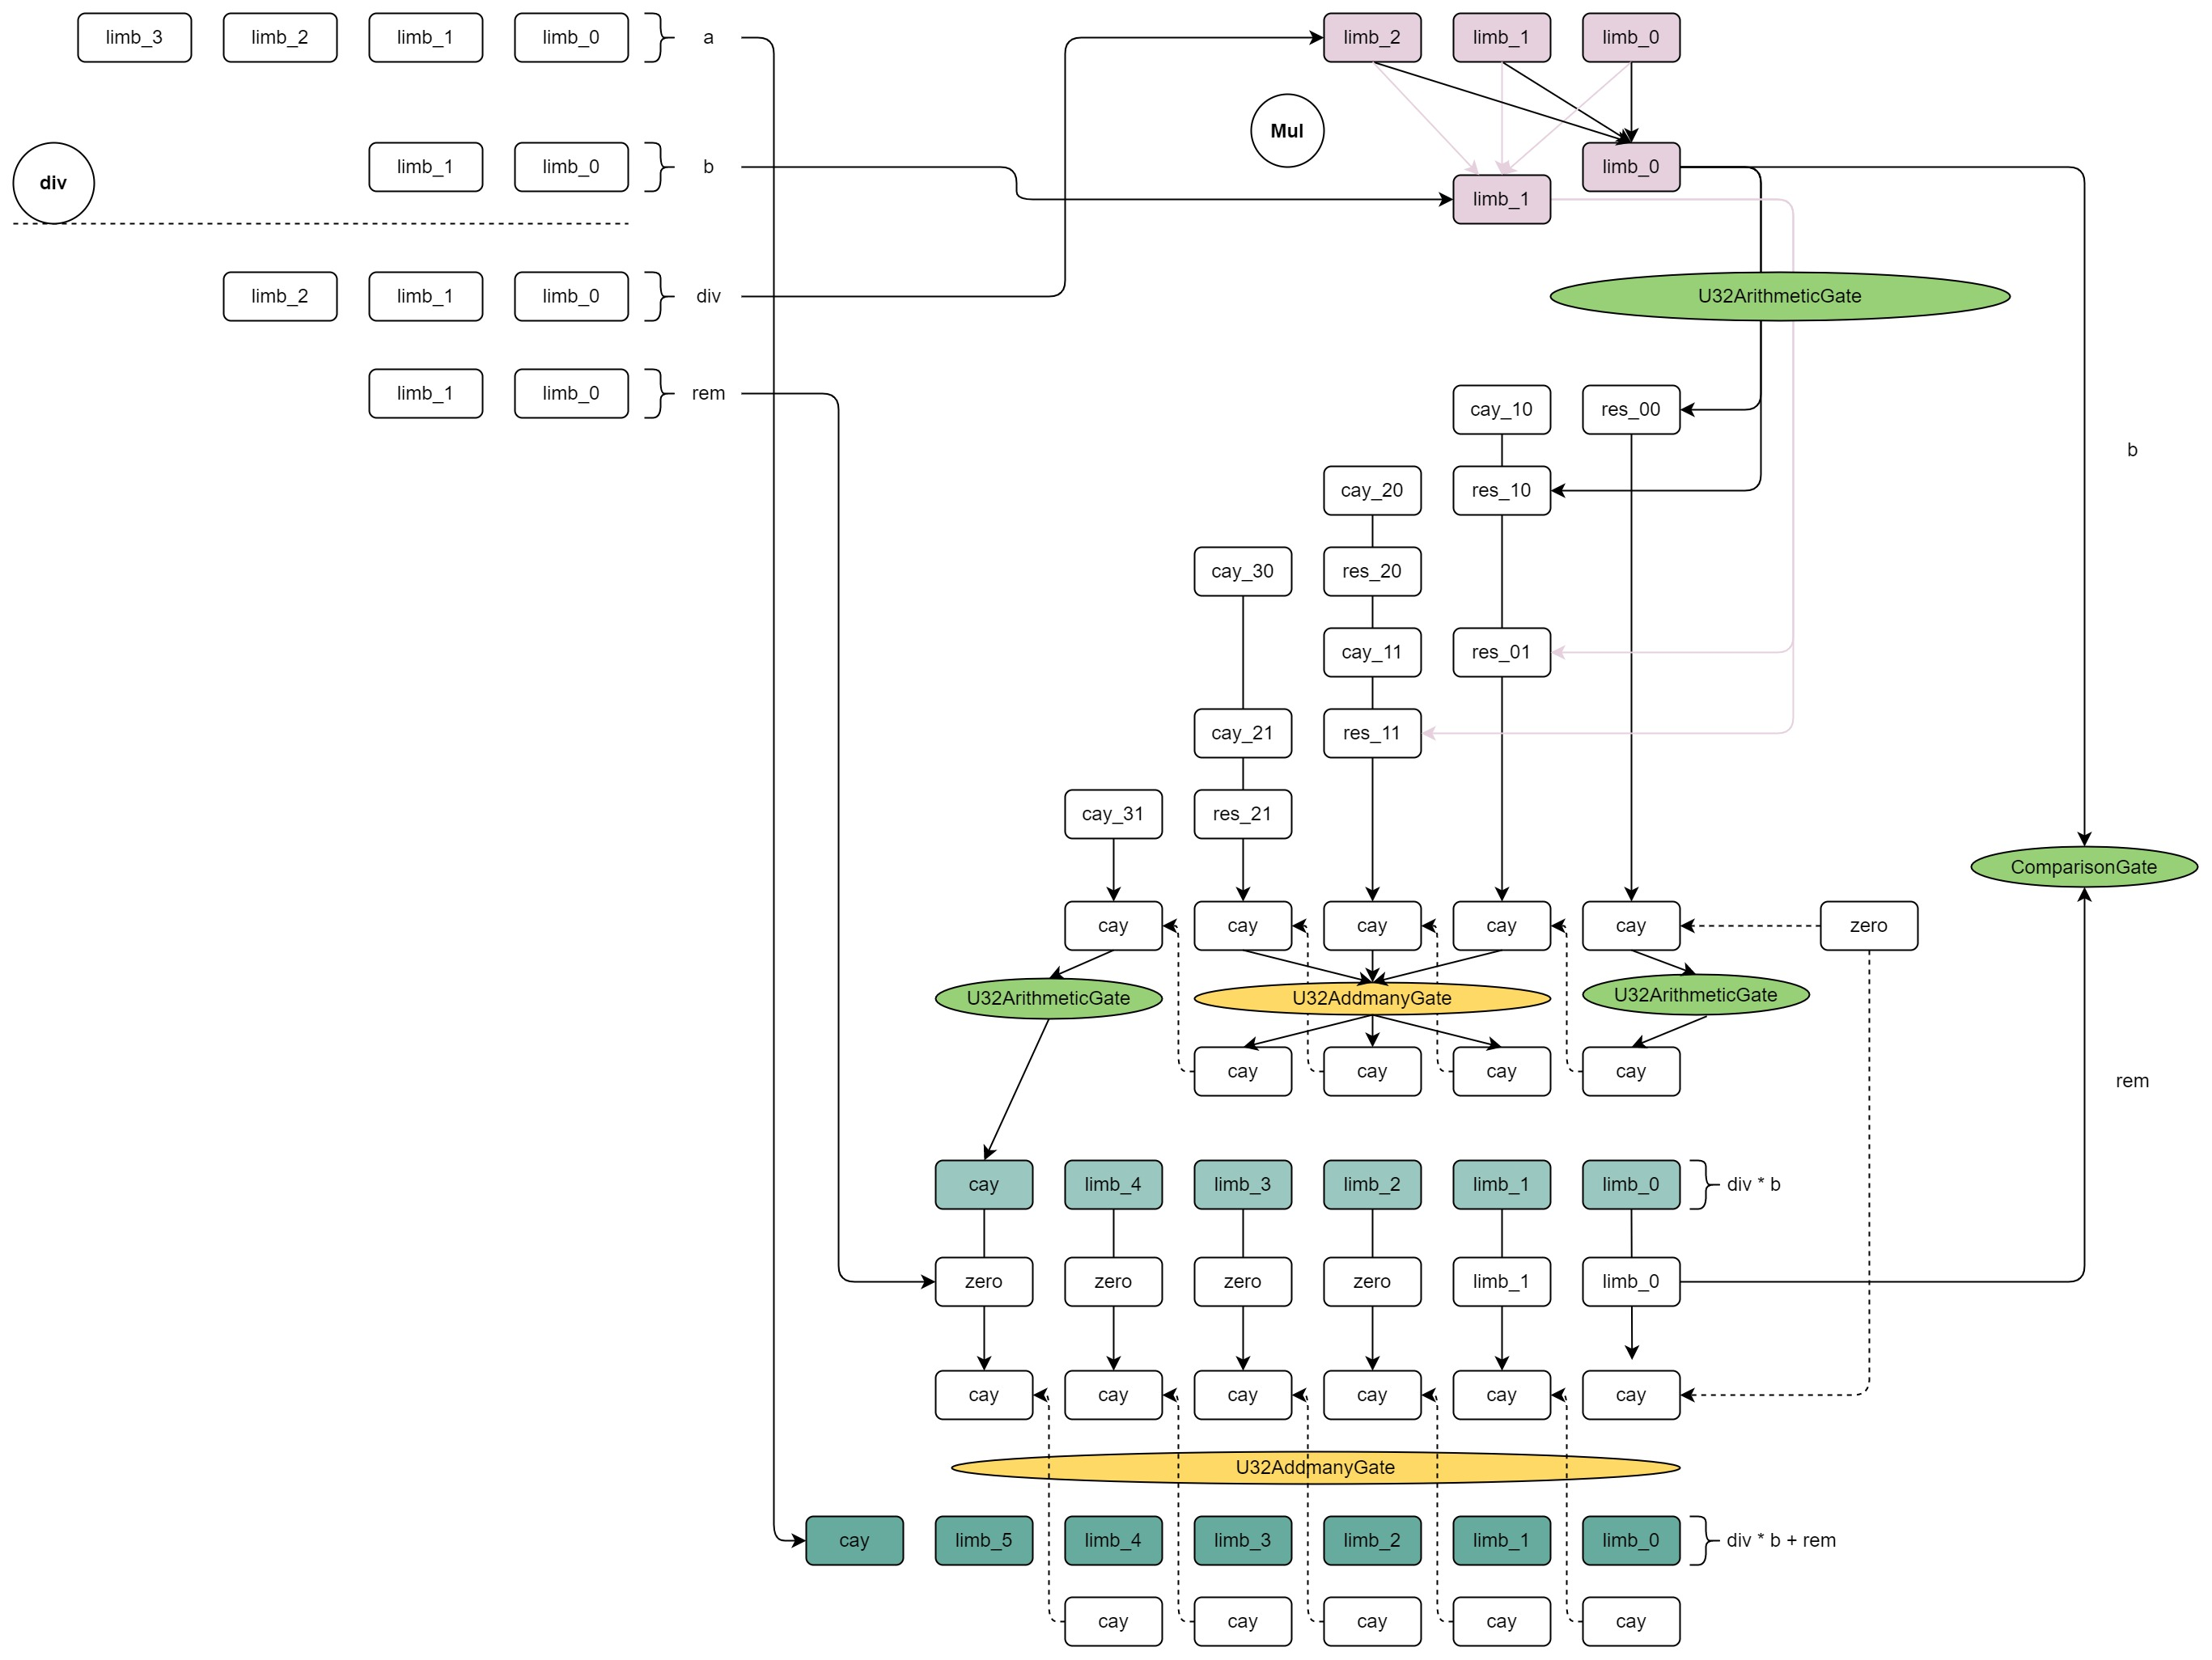
\includegraphics[width=0.6\textwidth]{biguint-div-layout.jpg}
    \caption{biguint-div layout}
    \label{fig:biguint-div-layout}
\end{figure}